% Pictogram for fig:setup (b): side view of the case stack at two heights under the same
% head camera. Hand-drawn TikZ (09-14); replaces a photo of the stack (images/Battery_stack.jpeg)
% per user preference. Drawn at final size (~36 mm wide) so labels stay legible; not to scale.
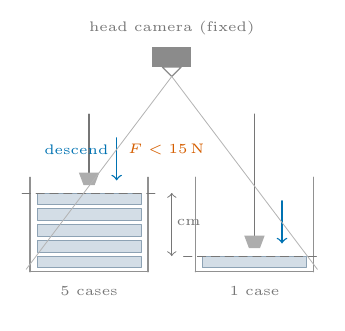
\begin{tikzpicture}[x=1mm, y=1mm, line cap=round, line join=round]
\definecolor{pgmuted}{HTML}{767676}
\definecolor{pgcase}{HTML}{9DB4C8}
\definecolor{pgcond}{HTML}{0072B2}
\definecolor{pgnaive}{HTML}{D55E00}
\useasboundingbox (-0.3,-4) rectangle (36.4,31);
% ---- two open boxes (side view) ----
\foreach \x/\n/\lab in {0/5/{5 cases}, 21/1/{1 case}} {
  \draw[pgmuted!80, line width=0.5pt] (\x,0) -- (\x+15,0) (\x,0) -- (\x,12) (\x+15,0) -- (\x+15,12);
  \foreach \i in {1,...,\n} {
    \fill[pgcase!45] (\x+0.9,{(\i-1)*2.0+0.5}) rectangle (\x+14.1,{\i*2.0});
    \draw[pgcase!90!black, line width=0.3pt] (\x+0.9,{(\i-1)*2.0+0.5}) rectangle (\x+14.1,{\i*2.0});
  }
  \node[font=\tiny, pgmuted, anchor=north] at (\x+7.5,-0.6) {\lab};
}
% ---- suction tool descending (arrow = commanded descent) ----
\foreach \x/\ytop in {0/10.0, 21/2.0} {
  \draw[pgmuted, line width=0.6pt] (\x+7.5,20) -- (\x+7.5,{\ytop+2.6});
  \fill[pgmuted!60] (\x+6.2,{\ytop+2.6}) -- (\x+8.8,{\ytop+2.6}) -- (\x+8.2,{\ytop+1.0}) -- (\x+6.8,{\ytop+1.0}) -- cycle;
  \draw[->, pgcond, line width=0.5pt] (\x+11,{\ytop+7}) -- (\x+11,{\ytop+1.6});
}
% ---- contact planes and their offset ----
\draw[pgmuted, densely dashed, line width=0.3pt] (-1,10) -- (16.5,10);
\draw[pgmuted, densely dashed, line width=0.3pt] (19.5,2) -- (37,2);
\draw[<->, pgmuted, line width=0.35pt] (18,10) -- (18,2);
\node[font=\tiny, pgmuted, anchor=west, inner sep=0.5pt] at (18.4,6.3) {cm};
% ---- stop-on-contact annotation ----
\node[font=\tiny, pgnaive, anchor=west, inner sep=0.5pt] at (12.2,15.5) {$F<15$\,N};
\node[font=\tiny, pgcond, anchor=east, inner sep=0.5pt] at (10.2,15.5) {descend};
% ---- head camera, same pose over both ----
\fill[pgmuted!85] (15.5,26) rectangle (20.5,28.6);
\draw[pgmuted!85, line width=0.4pt] (16.8,26) -- (19.2,26) -- (18,24.8) -- cycle;
\node[font=\tiny, pgmuted, anchor=south] at (18,28.8) {head camera (fixed)};
\draw[pgmuted!55, line width=0.3pt] (18,24.8) -- (-0.5,0.3);
\draw[pgmuted!55, line width=0.3pt] (18,24.8) -- (36.5,0.3);
\end{tikzpicture}
